%\documentstyle[epsf,twocolumn]{jarticle}       %LaTeX2.09仕様
%\documentclass[twocolumn]{jarticle}     %pLaTeX2e仕様
\documentclass{jarticle}     %pLaTeX2e仕様

%一枚組だったら[twocolumn]関係のとこ消す

\setlength{\topmargin}{-45pt}
%\setlength{\oddsidemargin}{0cm} 
\setlength{\oddsidemargin}{-7.5mm}
%\setlength{\evensidemargin}{0cm} 
\setlength{\textheight}{24.1cm}
%setlength{\textheight}{25cm} 
\setlength{\textwidth}{17.4cm}
%\setlength{\textwidth}{172mm} 
\setlength{\columnsep}{11mm}

\kanjiskip=.07zw plus.5pt minus.5pt

\usepackage{graphicx}
\usepackage[dvipdfmx]{color}
\usepackage{subcaption}
\usepackage{enumerate}
\usepackage{comment}
\usepackage{url}
\usepackage{multirow}
\usepackage{diagbox}
\usepackage{float}

\makeatletter
\newcommand{\figcaption}[1]{\def\@captype{figure}\caption{#1}}
\newcommand{\tblcaption}[1]{\def\@captype{table}\caption{#1}}
\makeatother



\begin{document}

  \noindent
  \onecolumn
  \hspace{1em}

  \today
  \hfill
  \ \  B3 西村昭賢 

  \vspace{2mm}
  \hrule
  \begin{center}
  {\Large \bf 情報工学実験2 10/25 課題}
  \end{center}
  \hrule
  \vspace{3mm}


\section{実験内容}
scikit-learnライブラリを用いて,様々な分類モデルを作成し,性能評価をした.

\subsection{データセット}
用いたデータセットはscikit-learnライブラリに組み込まれているIrisデータセットを用いた.
「花びらの長さ」,「花びらの幅」の2つの特徴量を用いて,Iris-setosa,Iris-versicolor,Iris-virginicaの3つのラベルをを0,1,2と整数で符号化したクラスラベルに対して分類をした.
\par
全体の30\%をテストデータ,その他70\%を学習データとしてデータセットをランダムに分割し実験をした.
データを分割する際,クラスラベルの比率は入力データセットと等しくなるようにした.

\subsection{用いたアルゴリズム}
分類モデルを作成する際,以下のアルゴリズムを用いた.

\begin{quote}
  \begin{itemize}
   \item パーセプトロン
   \item ロジスティック回帰
   \item 線形SVM
   \item カーネルSVM
   \item 決定木
   \item ランダムフォレスト
   \item k最近傍法
  \end{itemize}
 \end{quote}



\subsection{性能評価}

モデルの性能を評価する際,テストデータセットを用いて,以下の指標で評価した.

\begin{quote}
  \begin{itemize}
   \item 正解率(Accuracy)
   \item 適合率(Precision)
   \item 再現率(Recall)
   \item F1値(F1-measure)
   \item 混同行列(Confusion matrix)
  \end{itemize}
 \end{quote}
 適合率,再現率,F1値に関しては各クラスごと,分類結果全体の計算をした.
なお分類結果全体は,Irisデータセットにおいてラベルごとのデータの偏りは起こっていないためマクロ平均で計算した.\cite{macro}

\section{実験結果}
各アルゴリズムを用いたモデルに対し,前節で述べた性能評価をした結果を示す.以下,各モデルの正解率,適合率,再現率,F1値を示した表と,混同行列のヒートマップを示す.
\subsection{パーセプトロン}

\begin{figure}[h]
  \def\@captype{table}
  \begin{minipage}[c]{.48\textwidth}
    \tblcaption{パーセプトロンモデルにおける適合率,再現率,F1値,正解率}
      \label{table:パーセプトロン}
    \centering
      \begin{tabular}{lccc}
        \hline
        & Precision  &  Recall &  F1-measure \\
        \hline
        クラス0  & 0.93750  & 1.00000 & 0.96774 \\
        クラス1  & 1.00000  & 0.93333 & 0.96552 \\
        クラス2  & 1.00000  & 1.00000 & 1.00000 \\
        分類結果全体  &  0.97917  &  0.97778 & 0.97775 \\
        \hline
        Accuracy & & & 0.97778\\
        \hline
      \end{tabular}
  \end{minipage}
  %
  \hfill
  %
  \begin{minipage}[c]{.48\textwidth}
    \includegraphics[width=80mm]{assets/ppn_heatmap.eps}
    \caption{パーセプトロンモデルにおける混同行列のヒートマップ}
    \label{fig:パーセプトロン}
  \end{minipage}
\end{figure}


\subsection{ロジスティック回帰}

\begin{figure}[h]
  \def\@captype{table}
  \begin{minipage}[c]{.48\textwidth}
    \tblcaption{ロジスティック回帰モデルにおける適合率,再現率,F1値,正解率}
    \label{table:ロジスティック回帰}
    \centering
      \begin{tabular}{lccc}
        \hline
        & Precision  &  Recall &  F1-measure \\
        \hline
        クラス0  & 1.00000  & 1.00000 & 1.00000 \\
        クラス1  & 0.93750  & 1.00000 & 0.96774 \\
        クラス2  & 1.00000  & 0.93333 & 0.96552 \\
        分類結果全体  &  0.97917  &  0.97778 & 0.97775 \\
        \hline
        Accuracy & & & 0.97778\\
        \hline
      \end{tabular}
  \end{minipage}
  %
  \hfill
  %
  \begin{minipage}[c]{.48\textwidth}
    \includegraphics[width=80mm]{assets/lr_heatmap.eps}
  \caption{ロジスティック回帰モデルにおける混同行列のヒートマップ}
  \label{fig:ロジスティック}
  \end{minipage}
\end{figure}




\subsection{線形SVM}

\begin{figure}[H]
  \def\@captype{table}
  \begin{minipage}[c]{.48\textwidth}
    \tblcaption{線形SVMモデルにおける正解率,適合率,再現率,F1値}
    \label{table:線形SVM}
    \centering
      \begin{tabular}{lccc}
        \hline
        & Precision  &  Recall &  F1-measure \\
        \hline
        クラス0  & 1.00000  & 1.00000 & 1.00000 \\
        クラス1  & 0.93750  & 1.00000 & 0.96774 \\
        クラス2  & 1.00000  & 0.93333 & 0.96552 \\
        分類結果全体  &  0.97917  &  0.97778 & 0.97775 \\
        \hline
        Accuracy & & & 0.97778\\
        \hline
      \end{tabular}
  \end{minipage}
  %
  \hfill
  %
  \begin{minipage}[c]{.48\textwidth}
    \includegraphics[width=80mm]{assets/linear_heatmap.eps}
    \caption{線形SVMモデルにおける混同行列のヒートマップ}
    \label{fig:線形SVM}
  \end{minipage}
\end{figure}



\subsection{カーネルSVM}

\subsubsection{パラメータ$\gamma = 0.2$の時}

\begin{figure}[H]
  \def\@captype{table}
  \begin{minipage}[c]{.48\textwidth}
    \tblcaption{カーネルSVMモデルにおける正解率,適合率,再現率,F1値($\gamma = 0.2$)}
    \label{table:カーネルSVM}
    \centering
      \begin{tabular}{lccc}
        \hline
        & Precision  &  Recall &  F1-measure \\
        \hline
        クラス0  & 1.00000  & 1.00000 & 1.00000 \\
        クラス1  & 0.93750  & 1.00000 & 0.96774 \\
        クラス2  & 1.00000  & 0.93333 & 0.96552 \\
        分類結果全体  &  0.97917  &  0.97778 & 0.97775 \\
        \hline
        Accuracy & & & 0.97778\\
        \hline
      \end{tabular}
  \end{minipage}
  %
  \hfill
  %
  \begin{minipage}[c]{.48\textwidth}
    \includegraphics[width=80mm]{assets/kernel_heatmap.eps}
    \caption{カーネルSVMモデルにおける混同行列のヒートマップ($\gamma = 0.2$)}
    \label{fig:カーネル0.2SVM}
  \end{minipage}
\end{figure}

\subsubsection{パラメータ$\gamma = 100.0$の時}

\begin{figure}[H]
  \def\@captype{table}
  \begin{minipage}[c]{.48\textwidth}
    \tblcaption{カーネルSVMモデルにおける正解率,適合率,再現率,F1値($\gamma = 100.0$)}
    \label{table:カーネル100SVM}
    \centering
      \begin{tabular}{lccc}
        \hline
        & Precision  &  Recall &  F1-measure \\
        \hline
        クラス0  & 1.00000  & 0.93333 & 0.96552 \\
        クラス1  & 0.93333  & 0.93333 & 0.93333 \\
        クラス2  & 0.87500  & 0.93333 & 0.90323 \\
        分類結果全体  &  0.93611  &  0.93333 & 0.93403 \\
        \hline
        Accuracy & & & 0.93333\\
        \hline
      \end{tabular}
  \end{minipage}
  %
  \hfill
  %
  \begin{minipage}[c]{.48\textwidth}
    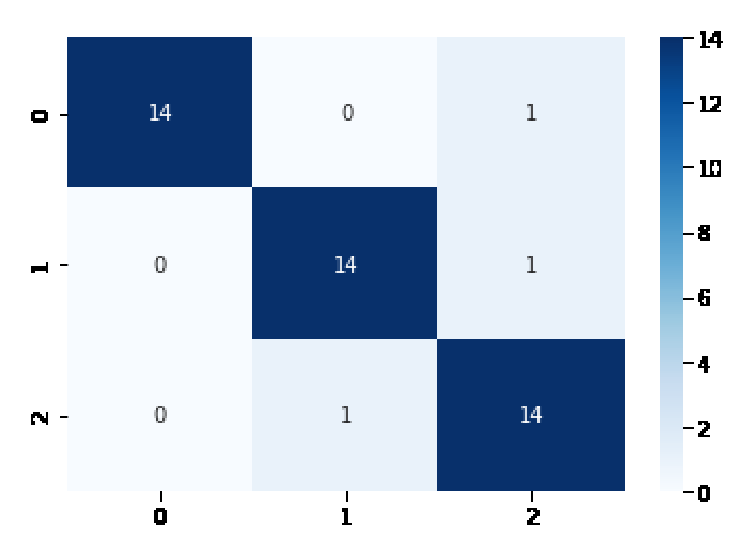
\includegraphics[width=80mm]{assets/kernel100_heatmap.eps}
    \caption{カーネルSVMモデルにおける混同行列のヒートマップ($\gamma = 100.0$)}
    \label{fig:カーネル100.0SVM}
  \end{minipage}
\end{figure}

\subsection{決定木}

\begin{figure}[H]
  \def\@captype{table}
  \begin{minipage}[c]{.48\textwidth}
    \tblcaption{決定木モデルにおける正解率,適合率,再現率,F1値(maxdepth = 4)}
    \label{table:決定木}
    \centering
      \begin{tabular}{lccc}
        \hline
        & Precision  &  Recall &  F1-measure \\
        \hline
        クラス0  & 1.00000  & 1.00000 & 1.00000 \\
        クラス1  & 0.93750  & 1.00000 & 0.96774 \\
        クラス2  & 1.00000  & 0.93333 & 0.96552 \\
        分類結果全体  &  0.97917  &  0.97778 & 0.97775 \\
        \hline
        Accuracy & & & 0.97778\\
        \hline
      \end{tabular}
  \end{minipage}
  %
  \hfill
  %
  \begin{minipage}[c]{.48\textwidth}
    \includegraphics[width=80mm]{assets/tree_heatmap.eps}
    \caption{決定木モデルにおける混同行列のヒートマップ(maxdepth = 4)}
    \label{fig:決定木}
  \end{minipage}
\end{figure}

\subsection{ランダムフォレスト}

\begin{figure}[H]
  \def\@captype{table}
  \begin{minipage}[c]{.48\textwidth}
    \tblcaption{ランダムフォレストモデルにおける正解率,適合率,再現率,F1値(n\_estimators = 25)}
    \label{table:ランダムフォレスト}
    \centering
      \begin{tabular}{lccc}
        \hline
        & Precision  &  Recall &  F1-measure \\
        \hline
        クラス0  & 1.00000  & 1.00000 & 1.00000 \\
        クラス1  & 0.93750  & 1.00000 & 0.96774 \\
        クラス2  & 1.00000  & 0.93333 & 0.96552 \\
        分類結果全体  &  0.97917  &  0.97778 & 0.97775 \\
        \hline
        Accuracy & & & 0.97778\\
        \hline
      \end{tabular}
  \end{minipage}
  %
  \hfill
  %
  \begin{minipage}[c]{.48\textwidth}
    \includegraphics[width=80mm]{assets/forest_heatmap.eps}
    \caption{ランダムフォレストモデルにおける混同行列のヒートマップ(n\_estimators = 25)}
    \label{fig:ランダムフォレスト}
  \end{minipage}
\end{figure}

\subsection{k最近傍法}

\begin{figure}[H]
  \def\@captype{table}
  \begin{minipage}[c]{.48\textwidth}
    \tblcaption{k最近傍法モデルにおける正解率,適合率,再現率,F1値(n\_neighbors=5)}
    \label{table:k最近傍法}
    \centering
      \begin{tabular}{lccc}
        \hline
        & Precision  &  Recall &  F1-measure \\
        \hline
        クラス0  & 1.00000  & 1.00000 & 1.00000 \\
        クラス1  & 1.00000  & 1.00000 & 1.00000 \\
        クラス2  & 1.00000  & 1.00000 & 1.00000 \\
        分類結果全体  &  1.00000  &  1.00000 & 1.00000 \\
        \hline
        Accuracy & & & 1.00000\\
        \hline
      \end{tabular}
  \end{minipage}
  %
  \hfill
  %
  \begin{minipage}[c]{.48\textwidth}
    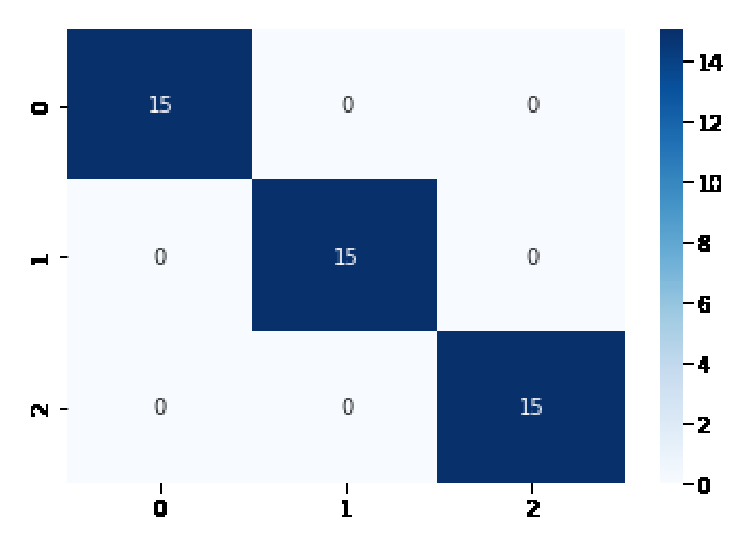
\includegraphics[width=80mm]{assets/kNN_heatmap.eps}
    \caption{k最近傍法モデルにおける混同行列のヒートマップ(n\_neighbors=5)}
    \label{fig:k最近傍法}
  \end{minipage}
\end{figure}




%index.bibはtexファイルと同階層に置く
%ちゃんと\citeしないと表示されない(1敗)
\bibliography{index.bib}
\bibliographystyle{junsrt}

\end{document}
